% \chapter{Plano de atividades para o próximo período}\label{chp:cronograma}

% As realizações foram apoiadas até o mês de agosto pelas reuniões e encontros virtuais semanais dos integrantes do laboratório e os médicos do CIREP, também orientadas pelas constantes buscas bibliográficas no estado da arte para realidade aumentada com \textit{Google Scholar} e \textit{IEEE}. Em especial, um artigo ajudou muito no início foi \textit{"Enhancing Reality: A Systematic Review of Augmented Reality in Neuronavigation and Education"\,} \cite{Cho2020}, que fez uma breve explicação da aplicabilidade da realidade aumentada em ambiente cirúrgico e compilou muitos resultados, tabelando precisão e equipamento utilizado.

% Dessa maneira, foi encontrado o artigo \textit{"Smart Glasses for Neurosurgical Navigation by Augmented Reality"\,} \cite{Maruyama2018}, que utilizou os óculos \textit{Moverio BT-200}, um modelo muito semelhante ao BT-350, para uma análise de sua aplicabilidade e precisão em neurocirurgias. Nesse trabalho, o programa exibe as projeções por meio do \textit{Unity} e a detecção é feita com ao menos duas câmeras que monitoram marcadores nos óculos e na cabeça do paciente. 

% \begin{figure}[ht]
%     \centering
%     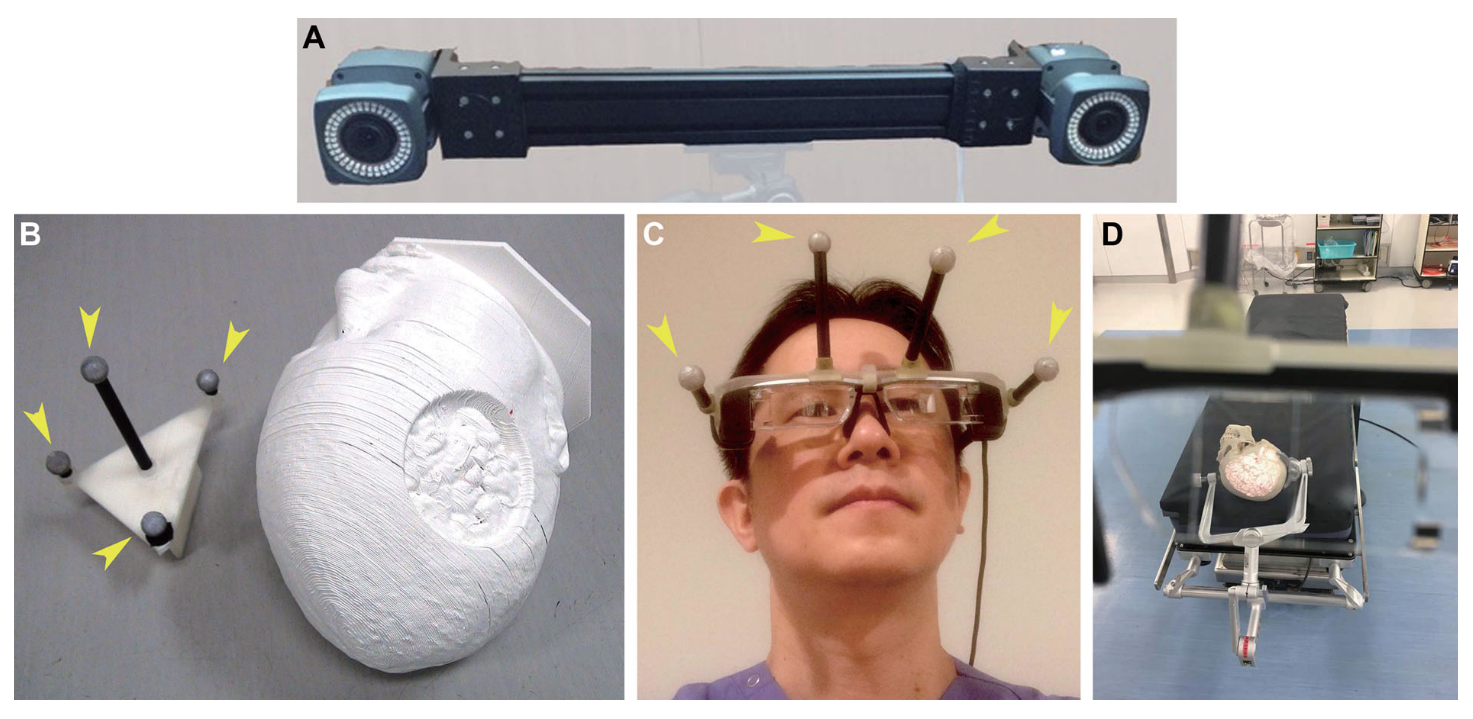
\includegraphics[width=.8\linewidth]{figuras/Maruyama.png}
%     \caption{(A) Duas câmeras para detectar movimento, (B) Marcadores para o paciente, (C) Marcadores nos óculos, (D) Visualização nos óculos. Fonte: \cite{Maruyama2018}}
%     \label{fig:Maruyama}
% \end{figure}

% Esse artigo conseguiu atingir a precisão na projeção de \((2,1 \pm 1,1 )mm\), um resultado excelente para a aplicação cirúrgica. Inspirando-se no método utilizado nesse artigo, planejamos também construir um sistema que só usa os óculos para a exibição das imagens geradas pelo computador, fazendo uma comunicação com conexão de rede local. Nesse aspecto, o projeto fica muito mais versátil pois a aplicação não depende dos recursos dos óculos e dá mais liberdade para o método e linguagem de programação na estimação de pose empregado na cabeça do paciente. 

% A ideia parece promissora e essa comunicação, do computador e os óculos com \textit{Unity}, já está em desenvolvimento. No computador, serão desenvolvidos algoritmos na linguagem \textit{Python} por termos um acesso melhor aos recursos de visão computacional e a implementação mais simplificada. Nos óculos, serão elaborados os métodos de interpretação das informações com lógica de programação por \textit{Socket} e exibição na tela do usuário.

% Uma proposta que trará uma mudança significativa para a importância do projeto é a ideia de integrar uma câmera sensível à profundidade: a \textit{Intel\textregistered \,RealSense\texttrademark\, Depth Camera D435i} \cite{Realsense}, disponibilizado como um recurso do laboratório. Por fim, o planejamento para os próximos seis meses até a conclusão do projeto é a comunicação da pose do paciente, vinda do computador aos óculos. Durante o processo, serão estudadas as possibilidades de arquitetura que podem-se configurar em um ambiente neurocirúrgico e utilização da \textit{Realsense}.

% \begin{figure}[ht]
%     \centering
%     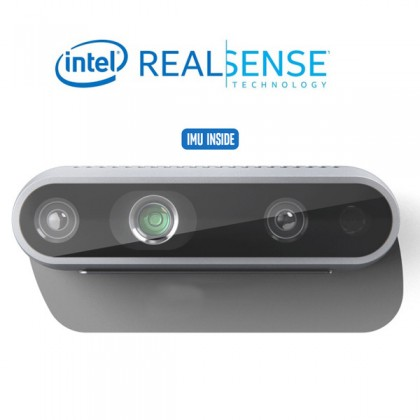
\includegraphics[width=.4\linewidth]{figuras/realsense.jpg}
%     \caption{Câmera com sensor de profundidade, \textit{RealSense\texttrademark \,D435i}. Fonte: \cite{Realsense}}
%     \label{fig:realsense}
% \end{figure}